\documentclass{article}

\usepackage{amsthm}
\usepackage{amsfonts}
\usepackage{amsmath}
\usepackage{amssymb}
\usepackage{fullpage}

\usepackage{graphicx}

\usepackage[usenames]{color}
\usepackage{hyperref}
  \hypersetup{
    colorlinks = true,
    urlcolor = blue,       % color of external links using \href
    linkcolor= blue,       % color of internal links 
    citecolor= blue,       % color of links to bibliography
    filecolor= blue,        % color of file links
    }
    
\usepackage{listings}

\definecolor{dkgreen}{rgb}{0,0.6,0}
\definecolor{gray}{rgb}{0.5,0.5,0.5}
\definecolor{mauve}{rgb}{0.58,0,0.82}

\lstset{frame=tb,
  language=haskell,
  aboveskip=3mm,
  belowskip=3mm,
  showstringspaces=false,
  columns=flexible,
  basicstyle={\small\ttfamily},
  numbers=none,
  numberstyle=\tiny\color{gray},
  keywordstyle=\color{blue},
  commentstyle=\color{dkgreen},
  stringstyle=\color{mauve},
  breaklines=true,
  breakatwhitespace=true,
  tabsize=3
}

\theoremstyle{theorem} 
   \newtheorem{theorem}{Theorem}[section]
   \newtheorem{corollary}[theorem]{Corollary}
   \newtheorem{lemma}[theorem]{Lemma}
   \newtheorem{proposition}[theorem]{Proposition}
\theoremstyle{definition}
   \newtheorem{definition}[theorem]{Definition}
   \newtheorem{example}[theorem]{Example}
\theoremstyle{remark}    
  \newtheorem{remark}[theorem]{Remark}


\title{CPSC 406}
\author{Tyler Lewis  \\ Chapman University}

\date{\today}

\begin{document}

\maketitle

\begin{abstract}
A very short introduction to typesetting in LaTeX for my courses ``Programming Languages'', ``Compiler Construction'' and ``Algorithm Analysis''.
\end{abstract}

\tableofcontents

\section{Homework}\label{intro}
\subsection{HW 1}

\begin{minipage}{0.4\textwidth}
\begin{itemize}
\item[\textbf{\emph{NFA2DFA}}] In order to convert the provided NFA to DFA I considered each possible combination of P, Q, R, and S, and considered each possible combination its own state. The included figure details every possible state the NFA/DFA may find itself in.
\end{itemize}
\end{minipage}%
%
\begin{minipage}{0.4\textwidth}
\begin{center}
    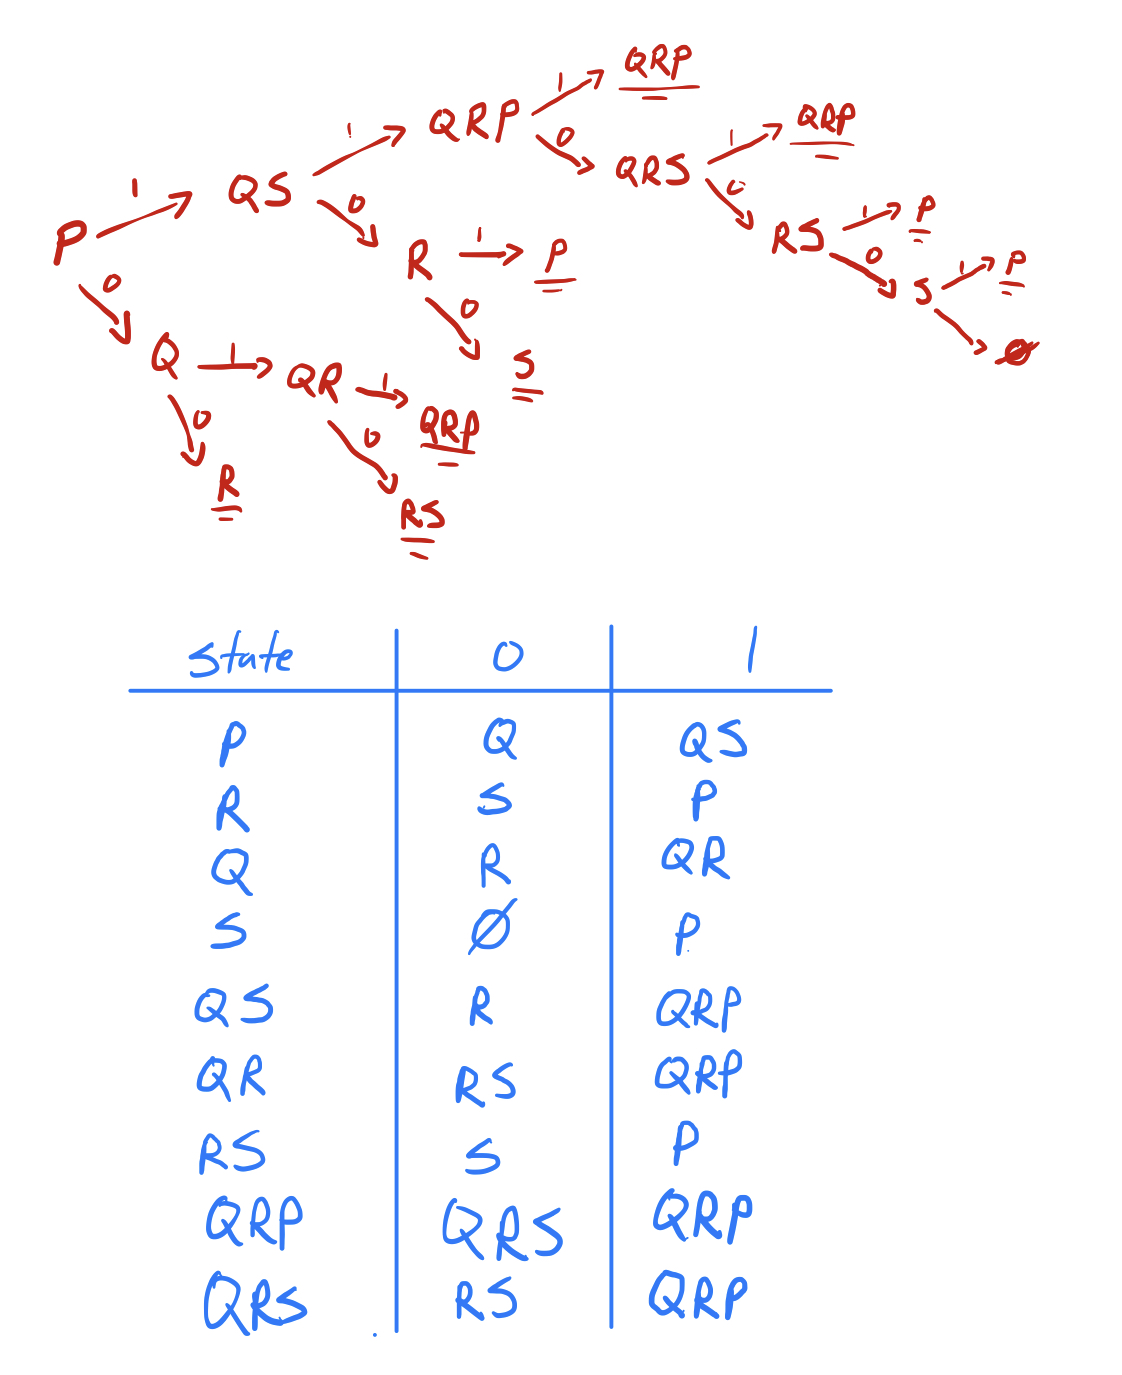
\includegraphics[width=\textwidth]{hw1.jpg}
    % \captionof{figure}{Gripper}
    \label{img:g}
\end{center}
\end{minipage}

\subsection{HW 2}

{\bf Question 1:}

    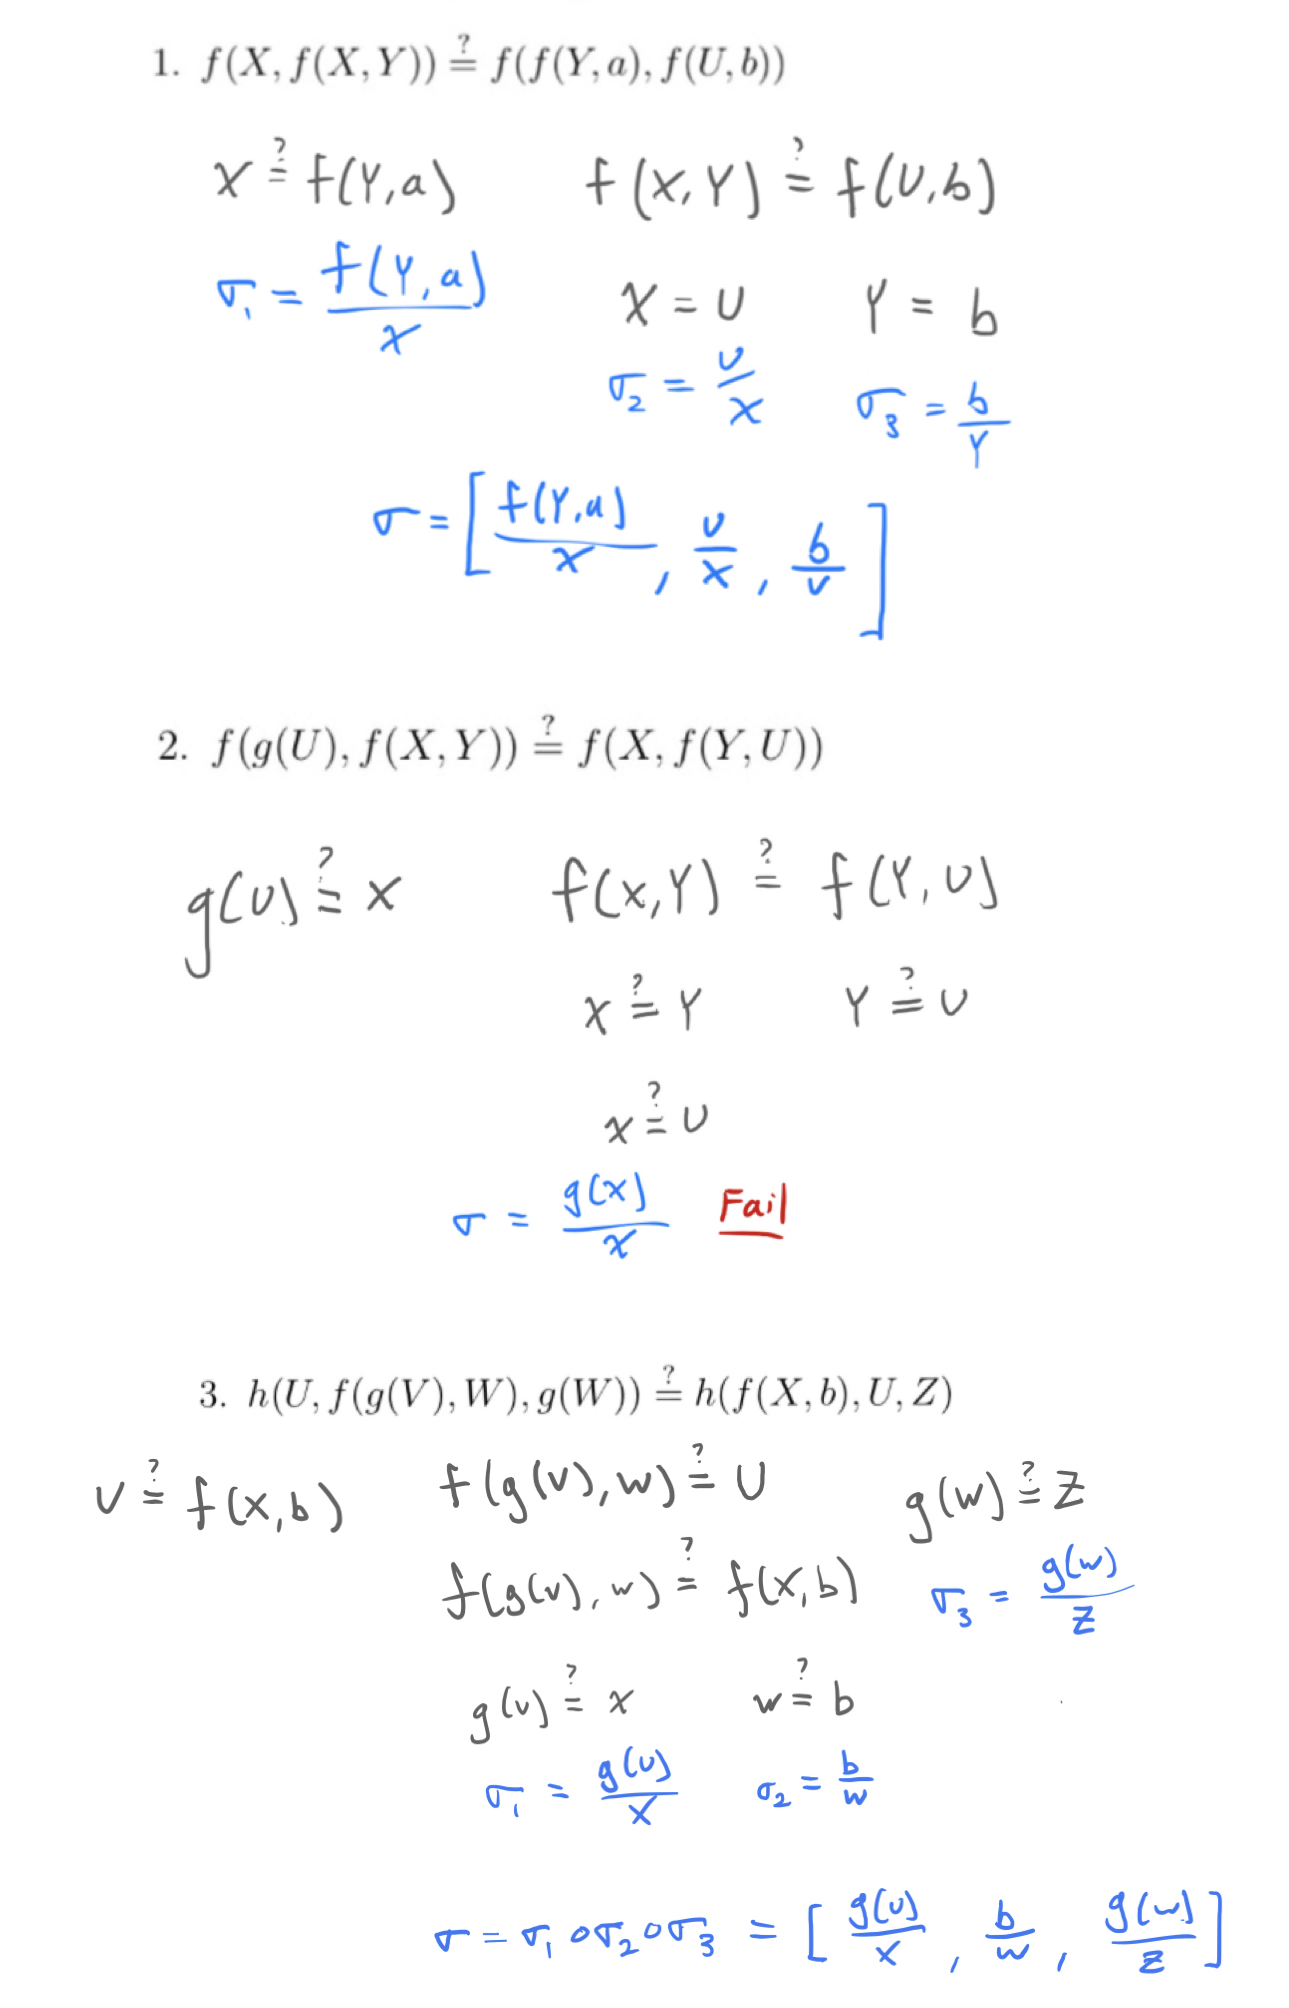
\includegraphics[width=10cm]{hw3q1.jpg}
    
% \end{center}
% \end{minipage}

{\bf Question 2:}
\texttt{
?- twoway(W,a)

?- conn(W,a), conn(a,W)

?- addr(W,a), addr(a,Z), serv(Z), addr(Z,W)
}

\subsection{HW 6}

    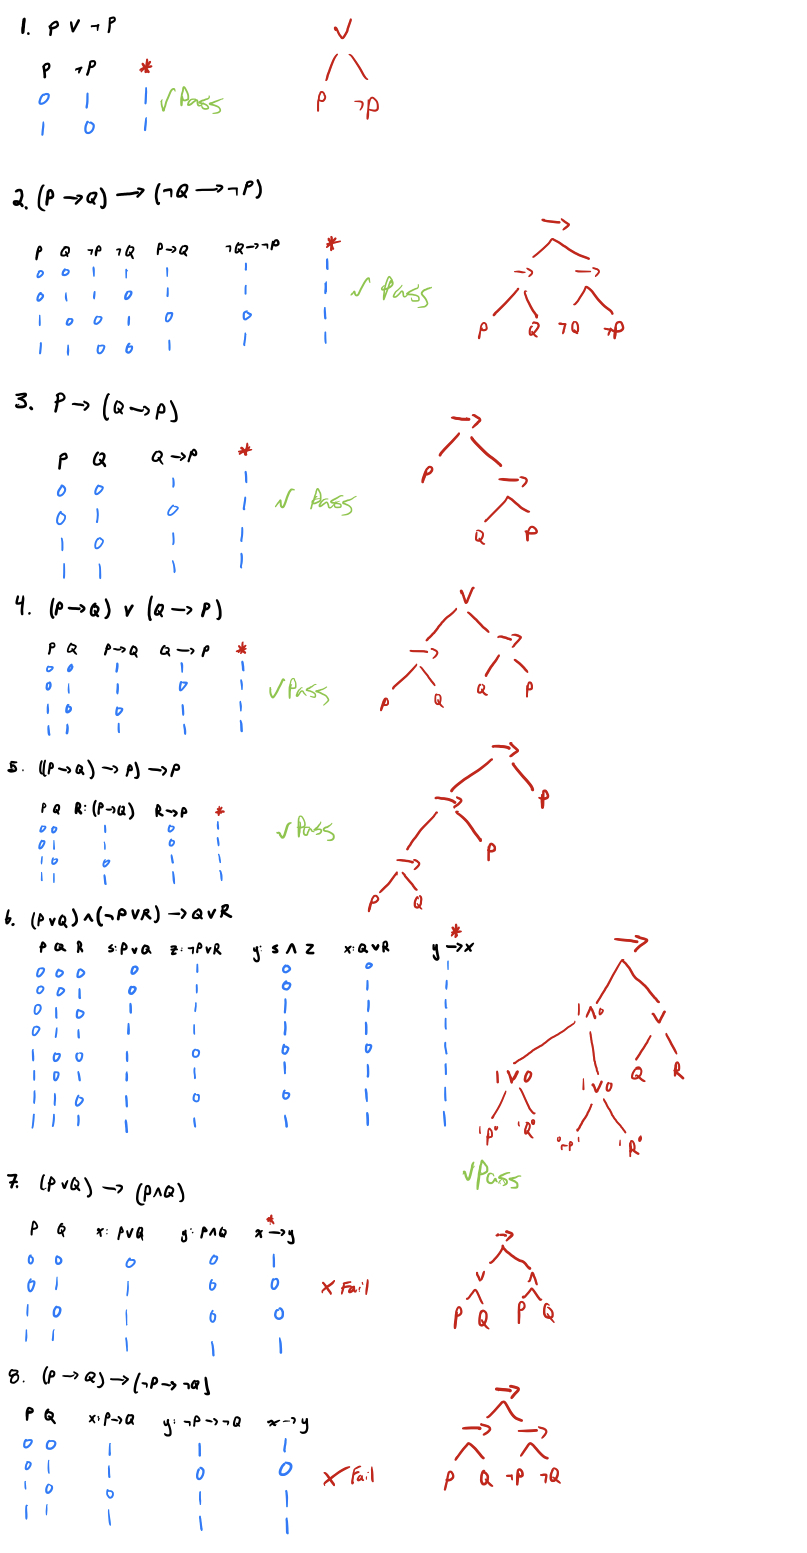
\includegraphics[width=9cm]{hw6.jpg}


\section{Conclusions}\label{conclusions}

In this document, to help you getting started, I gave a first succinct example of typesetting in Latex.

\begin{thebibliography}{99}
\bibitem[ALG]{Alg} \href{https://github.com/alexhkurz/algorithm-analysis-2023}{Algorithm Analysis}, Chapman University, 2023.
\end{thebibliography}

\end{document}
